%This section should describe the overall structure of your software system. Think of it as the strategy for how you will build the system. An architectural "layer" is the top-level logical view, or an abstraction, of your design. Layers should be composed of related elements of similar capabilities, and should be highly independent of other layers, but should have very clearly defined interfaces and interactions with other layers. Each layer should be identified individually and should be unique as to its function and purpose within the system. This section should also contain the high-level block diagram of the layers, as shown in the example below, as well as detailed descriptions of the functions of each layer.
The system consists of three major layers which are: The Daughter Board Layer, The Cypress CX3 Layer, and the Software Layer. The Daughter board is the main interface between the MIPI camera module and the Cypress CX3. It contains the OmniVision 5640 sensor that interfaces to the cypress CX3.
The Cypress CX3 layer provides the interface between the MIPI camera and the USB. This layer is what communicates with the computer and the Daughter board. It uses USB to power the device and transfer the data to a computer. 
The Software layer takes input from the Cypress Interface, processes that data, and tracks the pupil movement in real time. Various Computer Vision algorithms such as the Canny Edge Detector, Gaussian Smoothing, and the Random Sampling Consensus are implemented by the software layer to accurately track the pupil movement.



\begin{figure}[h!]
	\centering
 	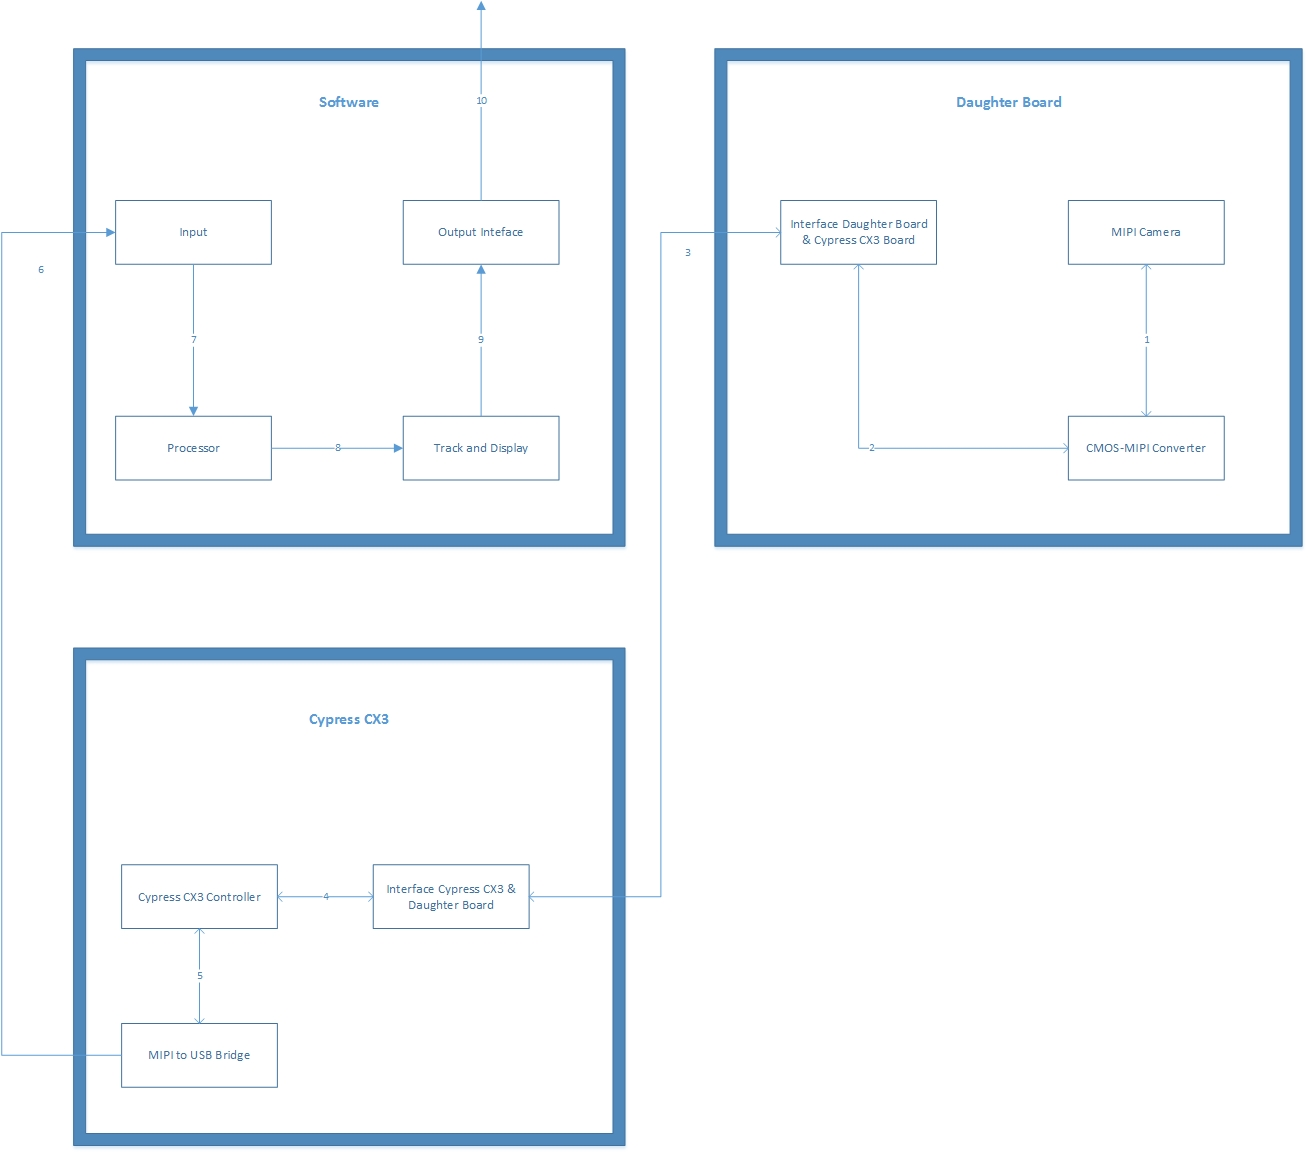
\includegraphics[width=0.60\textwidth]{images/Diagram_WHOLE.jpg}
 \caption{A simple architectural layer diagram}
\end{figure}

\subsection{Software Layer Description}
%Each layer should be described separately in detail. Descriptions should include the features, functions, critical interfaces and interactions of the layer. The description should clearly define the services that the layer provides. Also include any conventions that your team will use in describing the structure: naming conventions for layers, subsystems, modules, and data flows; interface specifications; how layers and subsystems are defined; etc. 
The software layer makes use of the OpenCV library and implements the entire program in C++ language. It consists of three major subsystems. The first subsystem is the Input subsystem. It gets input from the interface provided by the Cypress CX3. A video stream from a device (or a disk for test purposes) is read and stored into a CV::Mat structure. This structure will later be passed onto the processing subsystem.
The goal of the processing subsystem is to filter out all the noise (anything but the pupil) and it does so utilizing readily available OpenCV algorithms which shall be discussed in detail later in the document.
The final layer is the display layer which gathers information from the processor and displays the final result (fitted elipse) into the original video stream. 


\subsection{Daughter Board Description}
%Each layer should be described separately in detail. Descriptions should include the features, functions, critical interfaces and interactions of the layer. The description should clearly define the services that the layer provides. Also include any conventions that your team will use in describing the structure: naming conventions for layers, subsystems, modules, and data flows; interface specifications; how layers and subsystems are defined; etc. 
The daughter board is a board that is used to interface between the camera module 
and the Cypress CX3. This board uses a high-speed rugged ground plane socket 
(Base BRD Connector) to transfer the data that the camera captures to the CX3. In 
order for the camera module (pcDuino Camera Module) to function properly the 
daughter board needed a new camera connector, since the original connector is not 
compatible. We replaced the old connector with the Panasonic connector 
(AXK824145WG). The purpose of the new camera connector is to interface the 
camera with the Base BRD Connector. The daughter board contains the OmniVision 
5640 that is interfaced through the 2-lane MIPI interface.

\subsection{Cypress CX3 Description}
%Each layer should be described separately in detail. Descriptions should include the features, functions, critical interfaces and interactions of the layer. The description should clearly define the services that the layer provides. Also include any conventions that your team will use in describing the structure: naming conventions for layers, subsystems, modules, and data flows; interface specifications; how layers and subsystems are defined; etc. 
The Cypress CX3 is a MIPI to USB interface. This controller is fully functional with 
any image sensor that is compliant with a MIPI Camera Serial Interface (OmniVision 
5640). The Cypress CX3 is used to control the communication between a computer 
and the device, since it uses a USB connection to power the device and transfer the 
data that it collected. Also in order for the device to store the data read from the 
camera module, it uses EEPROMS in order to prevent loosing data in cases the 
device looses power. Then the device will transfer its data to the computer via USB. 
The Cypress CX3 is also connected to the MIPI camera.